%----------------------------------------------------------------------------------------
%	PACKAGES AND OTHER DOCUMENT CONFIGURATIONS
%----------------------------------------------------------------------------------------

\documentclass{tufte-book} % Use the tufte-book class which in turn uses the tufte-common class

% \hypersetup{colorlinks} % Comment this line if you don't wish to have colored links

\usepackage{microtype} % Improves character and word spacing

\usepackage{lipsum} % Inserts dummy text

\usepackage{booktabs} % Better horizontal rules in tables

\usepackage{graphicx} % Needed to insert images into the document
\graphicspath{{graphics/}} % Sets the default location of pictures
\setkeys{Gin}{width=\linewidth,totalheight=\textheight,keepaspectratio} % Improves figure scaling

\usepackage{fancyvrb} % Allows customization of verbatim environments
\fvset{fontsize=\normalsize} % The font size of all verbatim text can be changed here

\newcommand{\hangp}[1]{\makebox[0pt][r]{(}#1\makebox[0pt][l]{)}} % New command to create parentheses around text in tables which take up no horizontal space - this improves column spacing
\newcommand{\hangstar}{\makebox[0pt][l]{*}} % New command to create asterisks in tables which take up no horizontal space - this improves column spacing

\usepackage{xspace} % Used for printing a trailing space better than using a tilde (~) using the \xspace command

\usepackage{enumitem} % Used for hypothesis list

\newcommand{\monthyear}{\ifcase\month\or January\or February\or March\or April\or May\or June\or July\or August\or September\or October\or November\or December\fi\space\number\year} % A command to print the current month and year

\newcommand{\openepigraph}[2]{ % This block sets up a command for printing an epigraph with 2 arguments - the quote and the author
\begin{fullwidth}
\sffamily\large
\begin{doublespace}
\noindent\allcaps{#1}\\ % The quote
\noindent\allcaps{#2} % The author
\end{doublespace}
\end{fullwidth}
}

\newcommand{\blankpage}{\newpage\hbox{}\thispagestyle{empty}\newpage} % Command to insert a blank page

\usepackage{units} % Used for printing standard units

\newcommand{\hlred}[1]{\textcolor{Maroon}{#1}} % Print text in maroon
\newcommand{\hangleft}[1]{\makebox[0pt][r]{#1}} % Used for printing commands in the index, moves the slash left so the command name aligns with the rest of the text in the index
\newcommand{\hairsp}{\hspace{1pt}} % Command to print a very short space
\newcommand{\ie}{\textit{i.\hairsp{}e.}\xspace} % Command to print i.e.
\newcommand{\eg}{\textit{e.\hairsp{}g.}\xspace} % Command to print e.g.
\newcommand{\na}{\quad--} % Used in tables for N/A cells
\newcommand{\measure}[3]{#1/#2$\times$\unit[#3]{pc}} % Typesets the font size, leading, and measure in the form of: 10/12x26 pc.
\newcommand{\tuftebs}{\symbol{'134}} % Command to print a backslash in tt type in OT1/T1

\providecommand{\XeLaTeX}{X\lower.5ex\hbox{\kern-0.15em\reflectbox{E}}\kern-0.1em\LaTeX}
\newcommand{\tXeLaTeX}{\XeLaTeX\index{XeLaTeX@\protect\XeLaTeX}} % Command to print the XeLaTeX logo while simultaneously adding the position to the index

\newcommand{\doccmdnoindex}[2][]{\texttt{\tuftebs#2}} % Command to print a command in texttt with a backslash of tt type without inserting the command into the index

\newcommand{\doccmddef}[2][]{\hlred{\texttt{\tuftebs#2}}\label{cmd:#2}\ifthenelse{\isempty{#1}} % Command to define a command in red and add it to the index
{ % If no package is specified, add the command to the index
\index{#2 command@\protect\hangleft{\texttt{\tuftebs}}\texttt{#2}}% Command name
}
{ % If a package is also specified as a second argument, add the command and package to the index
\index{#2 command@\protect\hangleft{\texttt{\tuftebs}}\texttt{#2} (\texttt{#1} package)}% Command name
\index{#1 package@\texttt{#1} package}\index{packages!#1@\texttt{#1}}% Package name
}}

\newcommand{\doccmd}[2][]{% Command to define a command and add it to the index
\texttt{\tuftebs#2}%
\ifthenelse{\isempty{#1}}% If no package is specified, add the command to the index
{%
\index{#2 command@\protect\hangleft{\texttt{\tuftebs}}\texttt{#2}}% Command name
}
{%
\index{#2 command@\protect\hangleft{\texttt{\tuftebs}}\texttt{#2} (\texttt{#1} package)}% Command name
\index{#1 package@\texttt{#1} package}\index{packages!#1@\texttt{#1}}% Package name
}}

% A bunch of new commands to print commands, arguments, environments, classes, etc within the text using the correct formatting
\newcommand{\docopt}[1]{\ensuremath{\langle}\textrm{\textit{#1}}\ensuremath{\rangle}}
\newcommand{\docarg}[1]{\textrm{\textit{#1}}}
\newenvironment{docspec}{\begin{quotation}\ttfamily\parskip0pt\parindent0pt\ignorespaces}{\end{quotation}}
\newcommand{\docenv}[1]{\texttt{#1}\index{#1 environment@\texttt{#1} environment}\index{environments!#1@\texttt{#1}}}
\newcommand{\docenvdef}[1]{\hlred{\texttt{#1}}\label{env:#1}\index{#1 environment@\texttt{#1} environment}\index{environments!#1@\texttt{#1}}}
\newcommand{\docpkg}[1]{\texttt{#1}\index{#1 package@\texttt{#1} package}\index{packages!#1@\texttt{#1}}}
\newcommand{\doccls}[1]{\texttt{#1}}
\newcommand{\docclsopt}[1]{\texttt{#1}\index{#1 class option@\texttt{#1} class option}\index{class options!#1@\texttt{#1}}}
\newcommand{\docclsoptdef}[1]{\hlred{\texttt{#1}}\label{clsopt:#1}\index{#1 class option@\texttt{#1} class option}\index{class options!#1@\texttt{#1}}}
\newcommand{\docmsg}[2]{\bigskip\begin{fullwidth}\noindent\ttfamily#1\end{fullwidth}\medskip\par\noindent#2}
\newcommand{\docfilehook}[2]{\texttt{#1}\index{file hooks!#2}\index{#1@\texttt{#1}}}
\newcommand{\doccounter}[1]{\texttt{#1}\index{#1 counter@\texttt{#1} counter}}

\usepackage{makeidx} % Used to generate the index
\makeindex % Generate the index which is printed at the end of the document

% This block contains a number of shortcuts used throughout the book
\newcommand{\vdqi}{\textit{VDQI}\xspace}
\newcommand{\ei}{\textit{EI}\xspace}
\newcommand{\ve}{\textit{VE}\xspace}
\newcommand{\be}{\textit{BE}\xspace}
\newcommand{\VDQI}{\textit{The Visual Display of Quantitative Information}\xspace}
\newcommand{\EI}{\textit{Envisioning Information}\xspace}
\newcommand{\VE}{\textit{Visual Explanations}\xspace}
\newcommand{\BE}{\textit{Beautiful Evidence}\xspace}
\newcommand{\TL}{Tufte-\LaTeX\xspace}

%----------------------------------------------------------------------------------------
%	BOOK META-INFORMATION
%----------------------------------------------------------------------------------------

\title{Design and Evaluation of Spatial Interfaces in Virtual Reality} % Title of the book

\author[Tobias Bernard]{Tobias\ Bernard} % Author

\publisher{TU Berlin} % Publisher

%----------------------------------------------------------------------------------------

\begin{document}

\frontmatter


%----------------------------------------------------------------------------------------

\maketitlepage % Print the title page

%----------------------------------------------------------------------------------------
%	COPYRIGHT PAGE
%----------------------------------------------------------------------------------------

\newpage
\begin{fullwidth}
~\vfill
\thispagestyle{empty}
\setlength{\parindent}{0pt}
\setlength{\parskip}{\baselineskip}
Copyright \copyright\ \the\year\ \thanklessauthor

\par\smallcaps{Published by \thanklesspublisher}

\par\smallcaps{tufte-latex.googlecode.com}

\par Licensed under the Apache License, Version 2.0 (the ``License''); you may not use this file except in compliance with the License. You may obtain a copy of the License at \url{http://www.apache.org/licenses/LICENSE-2.0}. Unless required by applicable law or agreed to in writing, software distributed under the License is distributed on an \smallcaps{``AS IS'' BASIS, WITHOUT WARRANTIES OR CONDITIONS OF ANY KIND}, either express or implied. See the License for the specific language governing permissions and limitations under the License.\index{license}

\par\textit{First printing, \monthyear}
\end{fullwidth}

%----------------------------------------------------------------------------------------

\tableofcontents % Print the table of contents


\mainmatter

%----------------------------------------------------------------------------------------
%	ABSTRACT
%----------------------------------------------------------------------------------------

% \cleardoublepage
\chapter{Abstract}

In order to display more information than the screen can accomodate at any one time, traditional graphical user interfaces use clipping, \ie they employ a virtual space larger than the screen, which users can interactively navigate. Because users can only see a small part of the clipped data space at any given time, it is harder for them to establish a spatial model of the data. This can make interfaces difficult to navigate, especially with numbers of items.

Most Virtual Reality applications today employ the same clipping patterns as traditional 2D interfaces. It is our hypothesis that by using all the possibilities afforded by the 3D environment, usability in VR applications could be improved over clipping-based approaches.

We tested this hypothesis by displaying the same information (cards with monochrome icons) in different interfaces: One using 2D clipping, and two using 3D space to display the data. We found significantly increased performance in the spatial interfaces, as well as higher user satisfaction.



%----------------------------------------------------------------------------------------
%	INTRODUCTION
%----------------------------------------------------------------------------------------

% \cleardoublepage
\chapter{Introduction} % The asterisk leaves out this chapter from the table of contents

When displaying large amounts of information on any medium, whether it's a book, a paper map, or a phone's screen, there are always cases where it isn't possible to show everything at the same time. Strategies for handling this problem are as old as civilization: Ancient scrolls employ a single, linear surface which is rolled up, books split the information into chunks of similar size and put it on pages which can be stacked, and paper maps are be folded in intricate ways, in order to enable easy navigation in two dimensions (see figure~\ref{fig:falkmap}).

\begin{marginfigure}
\includegraphics[width=\linewidth]{falk-patent.png}
\caption{US Patent 2572460 \emph{``A United Method for Folding Maps and the Like''}, from 1951 by G. E. A. Falk, describes a technique for folding printed maps in such a way that they can be read without fully unfolding them.}
\label{fig:falkmap}
\end{marginfigure}

In screen-based graphical user interfaces, these cases are usually handled by relying on clipping, \ie by employing a virtual space on which all of the information is laid out, and cutting off the content at the edges of the screen. Users can then interactively navigate the virtual space by moving their viewport onto it, \eg by scrolling. This technique works, but it is suboptimal, because it puts the burden of keeping track of the position in the virtual space on the user. Instead of being able to see the entire space they have to rely on their mental model of it.

% It is not ideal, however, because content which is outside the viewport is completely invisible, and the user only has a rudimentary sense of position within the data space.
% they can take up the entire field of vision. However, since this field of vision is not infinitely large, there are still limits to how much data can be viewed at any one time. Since there are no natural boundaries in \textsc{vr}, it does not make sense to use clipping to hide the additional information.

Unlike with screens, there are no natural boundaries for Virtual Reality interfaces, because the virtual environment takes up the entire field of vision. Additionally, users can move around in this environment while using an application. This presents the opportunity to use this larger space, as well as the third dimension, in the design of user interfaces.

\begin{figure}
  \includegraphics{pinc.jpg}
  \caption{Mockup of a Virtual Reality interface covering the entire field of vision (hellopinc.com)}
  \label{fig:noboundaries}
\end{figure}

However, there are currently very few real-world examples of this kind of spatial interface in \textsc{vr}. Most applications are either games or novelty apps such as 3D drawing programs, likely because the resolution on the current generation of headsets is far too low for most productivity applications.
The interfaces with some complexity that do exist tend to mimic 2D interface patterns and employ letterboxing.

\begin{figure}
  \includegraphics{superhot.png}
  \caption{Application detail page in the Oculus Home store. Clicking the sections on the left changes the content of the center column with a fade animation.}
  \label{fig:superhot}
\end{figure}


In this study we explore spatial interfaces which enable the presentation and navigation of large data sets using the unique possibilities that 3D space affords. For example, instead of disappearing outside the viewport, list items can stack up on top of a list, shrink to a smaller size, or be arranged in a grid.

\begin{marginfigure}
  \includegraphics[width=\linewidth]{email.png}
  \caption{Prototype of a list interface which stacks overflowing cards in the z-dimension.}
  \label{fig:email}
\end{marginfigure}

\subsection{Reserach Question}
The primary research question is whether spatial interfaces can improve the usability of \textsc{vr} applications compared to clipping. Additionally, we are interested in the advantages and disadvantages of different spatial approaches.

To answer this question we built three different interfaces displaying the same data, two spatial, one employing clipping. We will then measure how efficient they are to navigate for our test subjects. In addition we will assess the hedonic qualities of the interfaces using a questionnaire.

\subsection{Contributions}
We will develop and evaluate general-purpose patterns for displaying and navigating large amounts of information in \textsc{vr}, which can be used by others building information-dense \textsc{vr} applications in the future. Some of our work may be applicable to 2D interfaces trying to avoid the negative effects of clipping as well.

\subsection{Outline}

.........


%----------------------------------------------------------------------------------------
%	RELATED WORK
%----------------------------------------------------------------------------------------

\chapter{Related Work}
\label{ch:related-work}

\section{Literature}
Academic research on virtual reality goes back as far as the 1980s.

\section{State of the Art VR Interfaces}
The current generation of VR Interfaces for productivity doesn't make much use of 3D space. Most interfaces are flat 2D panels, not very different from traditional 2D interfaces in both form and behavior. They rely heavily on flat, clipped, scrollable areas, or simply pagination with fade transitions.

We found this to be true on both Oculus and SteamVR, with Oculus making slightly better use of the 3D space by employing freely floating elements in space, while SteamVR's interface relies mostly on monolithic flat panels.
However, SteamVR has more consistent, spatial animations, while Oculus relies heavily on jarring cuts and fades.

\begin{figure}
  \includegraphics{steamstore.png}
  \caption{The SteamVR store interface is a single flat surface that behaves like a regular desktop app. On the bottom there is a taskbar to switch between open apps, and a system bar with time, volume and settings.}
  \label{fig:steamstore}
\end{figure}


\subsection{Controller-Mapped Interfaces}
One notable exception from the generally flat and traditional interfaces are the controls persistently mapped to the controllers in Google Earth and TiltBrush.

In Google Earth, there is a miniature globe fixed on top of the left hand controller. The right controller can be used to point at a position on the globe to teleport there. This kind of navigation with two hands feels very intuitive, because it only relies on direct hand movement in space, not abstract button mappings or external controls.

\begin{figure}
  \includegraphics{globe.png}
  \caption{The miniature globe is fixed to the top of the left hand controller and increases in size when pointed at by the right hand controller. A little red pin shows the location hovered by the cursor. Pressing the trigger button teleports to that location.}
  \label{fig:globe}
\end{figure}

In TiltBrush, the left hand has a persistent menu with three pages of settings, which are arrayed around the controller, facing outwards. They can be turned along the center axis with the left hand controller's touchpad, and the right hand controller is used to operate the menus.
The contents of the two menu panels not facing the user is not visible, likely so as not to be visually distracting. As the panels turn, only the one facing the user shows
The menus themselves are not as interesting as their containers, employing standard 2D interface patterns such as pagination and clipping.

In our opinion these examples show the potential of spatial interaces in VR, because they make use of the 3D space in a way that makes interfaces easier to navigate.

\begin{figure}
  \includegraphics{tiltbrushmenu.png}
  \caption{Color picker page, one of the three pages in the Tilt Brush menu}
  \label{fig:tiltbrushmenu}
\end{figure}


%----------------------------------------------------------------------------------------
%	PROTOTYPES
%----------------------------------------------------------------------------------------

\chapter{Prototypes}
\label{ch:prototypes}

\section{Technology}
The \textsc{VR} ecosystem is currently (mid 2017) still in its infancy. We experimented with the Oculus Rift \textsc{CV1} and the \textsc{HTC} Vive, both released in early 2016, and tested the headset and controller hardware, software ecosystem, and developer tools.

The installation and setup are very cumbersome for both headsets, especially on the software side, where we encountered many glitches, bugs, and usability problems.

The biggest issue with both headsets is the very low resolution, as both only have a resolution of $1080$ $\times$ $1200$px per eye. In addition, in the periphery of the display the picture is quite blurry, meaning that refocusing the eyes to the sides to see content there is not possible. This means that text needs to be either very big, or very close to be legible, and makes any kind of information-dense application impossible. This is exemplified by the fact that the visual entropy of most apps is roughly that of a smartphone. It is also likely the reason why there are currently only a handful of non-trivial, non-game applications available on both the Oculus store and Steam.

Both headsets do room scale tracking reasonably well, but we found the Vive tracking to be more reliable. This is likely due to its trackers being mounted higher up and on opposite sides of the room. Walking around in the roughly 2x2m space feels natural, but the limitations of being able to move only within such a small space quickly become clear in scenarios like games with open-world environments, where it means that teleporting has to be the primary means of movement.

\section{Development}
We developed our prototypes in WebVR using Mozilla's A-Frame Framework. A-Frame is a Javascript library which enables building VR experiences using declarative components directly in HTML. It runs completely standalone in the browser, and can be used with other Javascript libraries and standard web tooling. Though there are sometimes performance and stability issues, the quality of the experiences is more or less on par with native VR for simple applications.

\section{Prototype 1: Stacked List}
This prototype is a scrollable 1-dimensional list of cards which uses z-depth to stack overflow cards at both ends of a list. The content of these stacked cards is not visible, but their presence shows how many items there are above and below the currently visible cards, thereby intuitively communicating the position in the list to the user, without relying on external indicators (\eg scrollbars).

\begin{figure}
  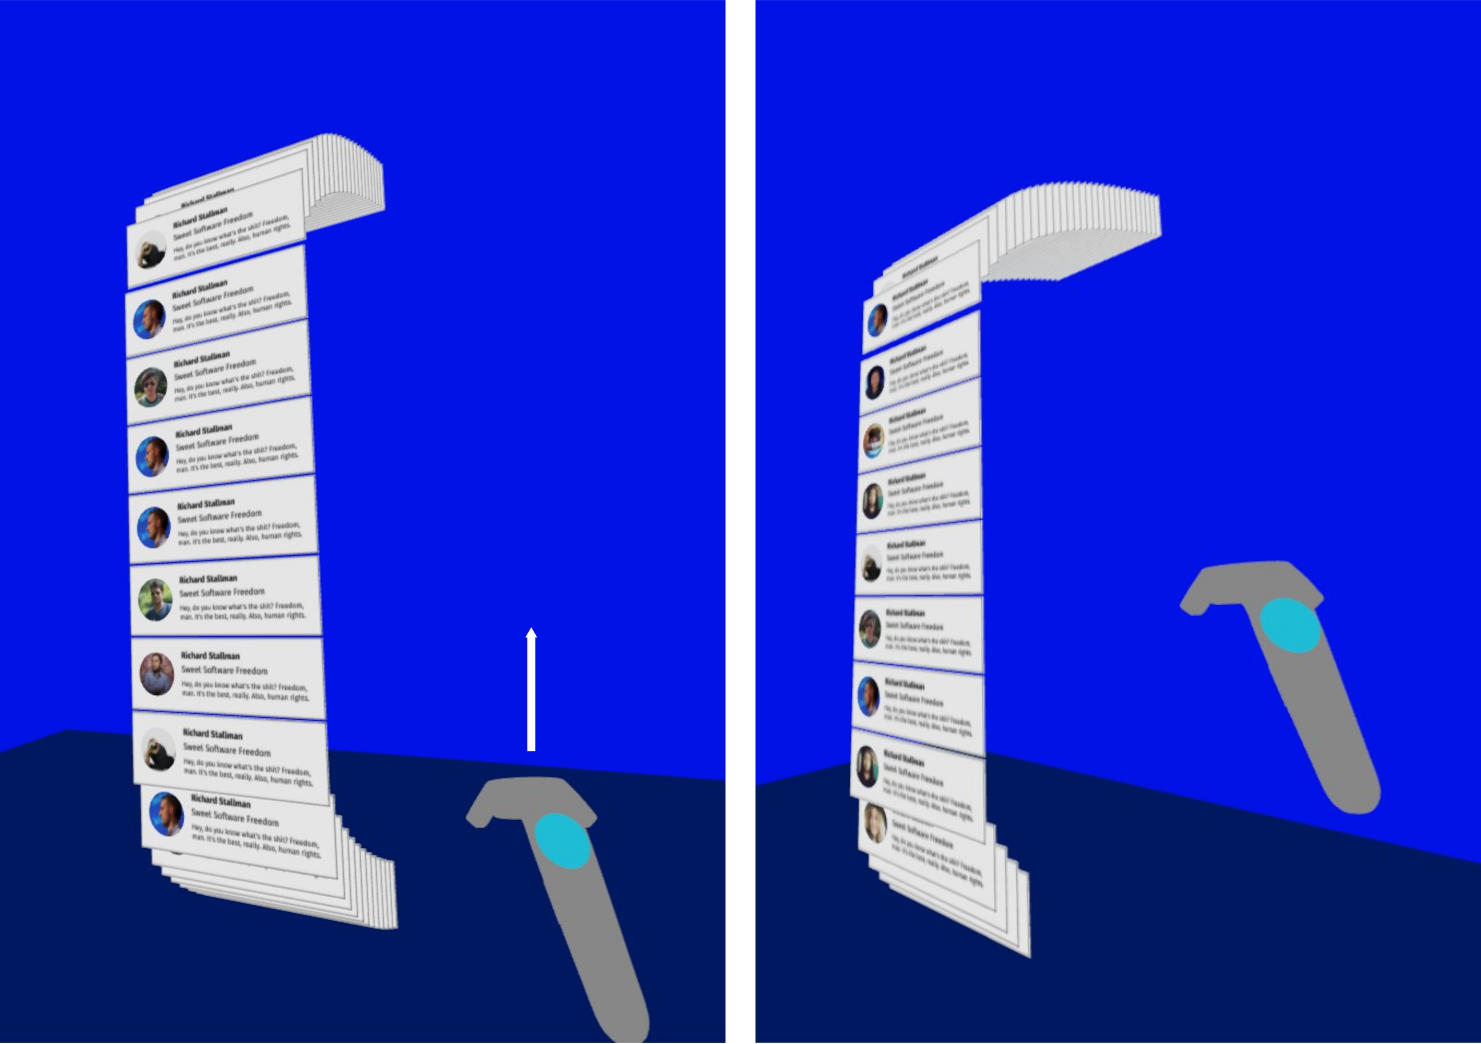
\includegraphics{emailscroll.png}
  \caption{Illustration of the scrolling behavior: Lifting up the controller while pressing the trigger button moves the cards up in the list.}
  \label{fig:emailscroll}
\end{figure}

Users can scroll the list by keeping the trigger button on the controller pressed while moving it vertically. The scrolling direction mimics the ``natural'' scrolling behavior on touchscreens and touchpads, whereby moving the controller up will move the elements upwards, thus scrolling down in the list.


\section{Prototype 2: Elevator}
This prototype is an attempt to use the available physical space as efficiently as possible, arraying information on a vertical 3D tube around the user. The information on the walls can be explored by walking around inside the tube, as well as changing the vertical position of the tube by ``scrolling'' it up and down.

\begin{figure}
  \includegraphics{picassoinside.jpg}
  \caption{The ``elevator'' prototype showing paintings on the walls of the cylinder. The vertical position can be moved by pressing the trigger button and moving the controller vertically.}
  \label{fig:picassoinside}
\end{figure}

\begin{marginfigure}
  \includegraphics[width=\linewidth]{picassooutside.jpg}
  \caption{The same prototype, seen from the outside}
  \label{fig:picassooutside}
\end{marginfigure}

%----------------------------------------------------------------------------------------
%	EXPERIMENTS
%----------------------------------------------------------------------------------------

\chapter{Study}
\label{ch:study}

To evaluate the differences between spatial and clipping-based interfaces we conducted an empirical study. We had participants perform the same task, finding icons in a list, using three different interfaces: A clipped, scrollable list, a scollable list that stacks overflowing elements in the z-dimension, and a two-dimensional grid.

\begin{figure}
  \includegraphics{types.png}
  \caption{The three different experiment types. Each of these was used in 6 different configurations, with different numbers of items, colored or monochrome.}
  \label{fig:experiement-types}
\end{figure}

\section{Participants}
We recruited 20 participants (8 female, 12 male), aged between 19 and 49 years (MDN = 24 years). Most of them were display workers, with an average of 5.9 hours per day working with computers (SD = 2.3 h). Most participants had some experience with Virtual Reality, but none of them had used it extensively.

\section{Apparatus}
The study was conducted in a university lab room using an HTC Vive connected to a Windows 10 PC. Participants were instructed to stand in the middle of an area measuring about $3m \times 3m$ at the center of the room. They were given the Vive headset and one tracked hand controller. The room-scale VR setup allowed them to freely move within this area and have their body and hand movement reflected faithfully inside VR.

\begin{figure}
\includegraphics{participant+view.png}
\caption{\emph{Left:} Participant standing at the designated spot in the middle of the room, wearing the Vive Headset and holding the controller. \emph{Right:} An experimental condition, as seen by the participant.}
\label{fig:participant-view}
\end{figure*}

\section{Design}
We used a within-subjects repeated measures design with three independent variables:

\begin{itemize}
  \item \emph{Interface type:} the three different interface types, \emph{Clipped}, \emph{Stacked}, and \emph{Spatial}
  \item \emph{Number of items:} 20, 50, or 250 icons
  \item \emph{Colored:} Whether all icons have the same white background, or different, colored backgrounds (from a palette of 10 colors)
\end{itemize}

The resulting 18 conditions were counterbalanced using a Latin square.

\begin{marginfigure}
  \includegraphics[width=\linewidth]{visual-field.png}
  \caption{Diagram of the human field of view}
  \label{fig:visual-field}
\end{marginfigure}

\subsection{Interface Types}

\emph{Spatial} is making use of the physical space to show all icons in a single grid. They can be navigated by simply moving one's head, and don't require additional interaction. The field of view taken up by this interface type varies from 45 to 100 degrees, depending on the number of icons.

\begin{figure*}[h]
\includegraphics[width=\linewidth]{fov-types.png}
\caption{Field of view for the different interface types}
\label{fig:fov-types}
\end{figure*}

\emph{Stacked} is a vertically scrolling single column of icons, where overflowing elements at the top and bottom of the column stack in the z-dimension. This means that all list elements are always present in the interface and are never completely hidden. Scrolling works by pressing and holding the trigger button and moving the controller up or down. This scrolls the list contiuously, following the vertical movement of the controller.

\emph{Clipped} is similar to \emph{Stacked}, except overflowing items disappear instead of stacking. The list is "clipped" at the top and bottom. The scrolling interaction is the same as for \emph{Stacked}.

\begin{figure*}[h]
\includegraphics[width=\linewidth]{interface-types.png}
\caption{The three different interface types (left to right): Spatial, Stacked, and Clipped}
\label{fig:interface-types}
\end{figure*}


\subsection{Number of Items}

The three different list sizes (20, 50, and 150) were chosen to test the entire spectrum of list sizes that realistically appear in user interfaces. 150 was chosen as the largest size because with more items, participants in our pilot studies quickly became frustrated by the long distances they had to scroll.

\begin{marginfigure}
  \includegraphics[width=\linewidth]{controllers.png}
  \caption{The 5 icons fixed to the left of the controller were used to guide the participants through the experiment. During each task, the current target icon was highlighted, the others were black. Selecting the target icon would reveal the next target icon on the controller, and obscure the previous one.}
  \label{fig:controllers}
\end{marginfigure}

\subsection{Colored/Monochrome}

We included the \emph{Colored} variable in order to understand the differences between \emph{Clipped} and \emph{Stacked} better. When all icons have the same background color, it is not possible to see what icons are on the "stacked" cards at both ends of the list. With different background colors, they can at least be differentiated when they are stacked, even though the actual icons are still obscured. We chose a palette of 10 colors that are each assigned to 10\percent of the total number of icons. In additon, we also tested all conditions in a monochrome variant, where the background is white for all icons.

\subsection{Tasks}
The interfaces in all conditions display a number of squares with simple monochrome icons. Participants had to find specific icons, one at a time. The icon set used is a subset of the Material Design icon set used by Android and other Google products.

\begin{marginfigure}
  \includegraphics[width=\linewidth]{material-icons.png}
  \caption{Examples of the icons used in the experiments}
  \label{fig:material-icons}
\end{marginfigure}

\emph{Initial:} First, participants had to find 5 icons, which were pseudo-randomly distributed across the entire set (one icon per quintile). To select the icon, they had to point at it with the raycasting cursor starting from the top of their controller, and press the trigger button.

\emph{Repeat:} After finding each icon once, participants had to find the same 5 icons again, but in randomized order. Each participant had to find and select a total of 180 icons ($18$ conditions $\times$ $(5 + 5) $ icons).

\subsection{Hypotheses}
One of our hypotheses in performing the experiments was that \emph{Spatial} would show the highest task performace for both \emph{Initial} and \emph{Repeat}, since the entire set of icons is visible and can be explored by simply looking around the room. This gives the interface an advantage over the other types both for initial discovery (less interaction required) and re-discovery in the second task (due to spatial memory).

Due to the similarities in structure and interaction, we assumed that \emph{Clipped} and \emph{Stacked} would perform similarly for \emph{Initial}.
For \emph{Repeat Colored}, we hypothsized that \emph{Stacked} would show higher performance than \emph{Clipped}, because it does not hide elements completely, but stacks them in space, giving participants a clearer sense of their position in the list and making it easier to find icons again.

Therefore, our hypotheses are the following:

\begin{enumerate}[label=H\arabic*. , wide=0.5em,  leftmargin=*]
  \item \emph{Spatial} outperforms \emph{Clipped} and \emph{Stacked}
  \item \emph{Repeat} outperforms \emph{Initial}
  \begin{enumerate}[label=H2.\arabic*. , wide=0.5em,  leftmargin=*]
    \item \emph{Clipped} and \emph{Stacked} perform similarly for \emph{Initial}
    \item \emph{Stacked} outperforms \emph{Clipped} for \emph{Repeat Colored}
  \end{enumerate}
  \item \emph{Colored} outperforms \emph{Monochrome}
\end{enumerate}

\section{Procedure}
Participants were given a demographic questionnaire, and then introduced to the VR setup. They put on the headset and were handed the controller. They then received instructions for how to use the interfaces in the experiment from a short tutorial in VR. The tutorial consists of two parts.
In the first part the participants were shown how to select icons using the right controller's raycasting cursor.

\begin{figure}
  \includegraphics{tutorials.png}
  \caption{The five initial steps of the experiment, including 2 tutorial and 3 example steps}
  \label{fig:tutorials}
\end{figure}

In the second part they were shown how to scroll in \emph{Clipped} and \emph{Stacked} interfaces, by keeping the trigger button pressed and moving the controller vertically.
Participants were told to perform the tasks \emph{as quickly as possible without making any errors}.

After being introduced to the basic interactions, participants got 3 example conditions (one for each interface type). This allowed them to learn the mechanics and get comfortable with the different interfaces before the actual experiment.

Then they performed the tasks for all 18 conditions, counterbalanced using a Latin square. After each condition, they had to answer a questionnaire with four qualitative statements assessing their experience with a given condition. Participants rated each of the statements on a 7-point Likert scale (1 = not true at all, 7 = very true).

These are the four statements:

\begin{enumerate}[label=\arabic*. , wide=0.5em,  leftmargin=*]
  \item I could memorize the position of the items.
  \item I was overwhelmed by the number of items.
  \item I found the layout efficient to navigate.
  \item I could easily find the item I was looking for.
\end{enumerate}

After the experiment, which lasted about 45 minutes, participants were given a questionnaire rating the three interface types (both color and monochrome) on a 7-point Likert scale (1 = very negatively, 7 = very positively).

\section{Data Collection}
For each condition, we logged the time participants took to select each icon. We also logged selection errors (selection of non-target icons), scroll distances for \emph{Clipped} and \emph{Stacked} conditions, and controller movement in the room throughout the experiments.

%----------------------------------------------------------------------------------------
%	RESULTS
%----------------------------------------------------------------------------------------

\chapter{Results}
\label{ch:results}




%----------------------------------------------------------------------------------------
%	DISCUSSION
%----------------------------------------------------------------------------------------

\chapter{Discussion}
\label{ch:discussion}


......

%----------------------------------------------------------------------------------------
%	CONCLUSION
%----------------------------------------------------------------------------------------

\chapter{Conclusion}
\label{ch:conclusion}


......

%----------------------------------------------------------------------------------------

\backmatter

%----------------------------------------------------------------------------------------
%	BIBLIOGRAPHY
%----------------------------------------------------------------------------------------

\bibliography{bibliography} % Use the bibliography.bib file for the bibliography
\bibliographystyle{plainnat} % Use the plainnat style of referencing

%----------------------------------------------------------------------------------------

\printindex % Print the index at the very end of the document

\end{document}
